%
%
%در این فایل، فصل اول پایان‌نامه خود را وارد کنید.
%
%
\chapter{
عنوان فصل اول را وارد کنید  
}\label{chap1} 

مطالب فصل اول را وارد کنید.

\section{
عنوان بخش اول را وارد کنید  
}\label{sec11} 

یک نمونه شکل در پایین:

\begin{figure}
\centering
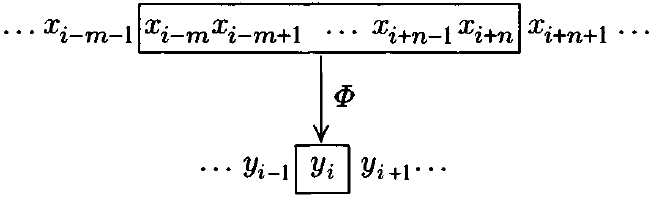
\includegraphics[scale=0.6]{S1}
\caption{بلوک کد لغزنده}
\label{Slide}
\end{figure}

ارجاع به شکل هم بصورت زیر است: شکل~\ref{Slide} را ببینید.
مطالب بخش اول را وارد کنید.

\section{
عنوان بخش دوم را وارد کنید  
}\label{sec12} 

مطالب بخش دوم را وارد کنید. یک نمونه جدول
\begin{table}
\caption{براورد پارامترهای دو مدل در برازش به داده‌های بقای سانسور 1 \label{TabAa31}}%
\centering
%\scriptsize
\begin{tabular}{cccccccccc}
\\
\hline 
		&	&      &     \multicolumn{7}{c}{تعداد تکرار}\\
\cline{4-10}
درصد		&	&      &     \multicolumn{3}{c}{500} & & \multicolumn{3}{c}{1000}\\
\cline{4-6} \cline{8-10}
سانسور & مدل & پارامتر &  براورد & $MAPB$ & $MSE$ & & براورد & $MAPB$ & $MSE$ \\
\hline
\multirow{6}{*}{20} &
	& $\beta_1$ & 0/504 & 3/969 & 0/0006 & & 0/503 & 3/967 & 0/0006 \\
&کاکس& $\beta_2$ & 0/617 & 14/771 & 0/0125 & & 0/610 & 15/277 & 0/0129 \\
\vspace{2mm}
&	& $\beta_3$ & 0/704 & 5/409 & 0/0022 & & 0/703 & 5/585 & 0/0025 \\
&	& $\beta_1$ & 0/518 & 5/503 & 0/0013 & & 0/517 & 5/490 & 0/0013 \\
&شکنندگی & $\beta_2$ & 0/633 & 16/045 & 0/0148 & & 0/626 & 16/322 & 0/0150  \\
\vspace{2mm}
&	& $\beta_3$ & 0/724 & 6/741 & 0/0037 & & 0/723 & 6/919 & 0/0039 \\
\multirow{6}{*}{40} &
	& $\beta_1$ & 0/504 & 4/435 & 0/0007 & & 0/504 & 4/369 & 0/0008 \\
&کاکس& $\beta_2$ & 0/612 & 16/677 & 0/0157 & & 0/607 & 17/009 & 0/0163 \\
\vspace{2mm}
&	& $\beta_3$ & 0/705 & 6/405 & 0/0031 & & 0/705 & 6/629 & 0/0034 \\
&	& $\beta_1$ & 0/520 & 6/109 & 0/0015 & & 0/520 & 6/050 & 0/0016 \\
&شکنندگی & $\beta_2$ & 0/631 & 18/128 & 0/0184 & & 0/625 & 18/186 & 0/0187 \\
\hline
\end{tabular}
\end{table}